\documentclass[a4paper,11pt]{article}
\usepackage[utf8]{inputenc}
\usepackage[english]{babel}
\usepackage{subfigure}
\usepackage{epsfig}
\usepackage{graphicx,url}
\usepackage{verbatim}
\usepackage{cite}
\usepackage{psfrag}
\usepackage{alltt}
\usepackage{vmargin}
\usepackage{indentfirst}
\usepackage{picins}

\setmargnohfrb{25mm}{25mm}{25mm}{25mm}

\begin{document}


\parpic{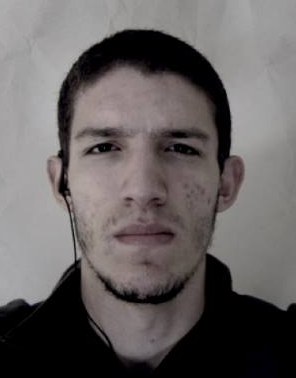
\includegraphics[width=1.2in,clip,keepaspectratio]{photos/nicollas.png}}
~\\
\textbf{Nicollas Rodrigues de Oliveira} is currently a PhD student in Telecommunications Engineering at Universidade Federal Fluminense. He got his master's degree in Telecommunications Engineering from Universidade Federal Fluminense (UFF) in 2020, and he graduated in Telecommunications Engineering at the same university in 2018. Between 2016 and 2018, he was a volunteer student, and later, he was a scholarship holder for a scientific initiation project. 

\vspace{1cm}

\parpic{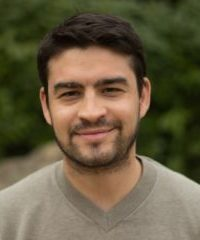
\includegraphics[width=1.2in,clip,keepaspectratio]{photos/martin.jpg}}
~\\
\textbf{Martin Andreoni Lopez} is a researcher of the Secure Systems Research Centre (SSRC) at Technology Innovation Institute (TII), United Arab Emirates. He graduated as an Electronics Engineer from \textit{Universidad Nacional de San Juan} (UNSJ), Argentina, in 2011. He got his Master's degree in Electrical Engineering from the \textit{Universidade Federal do Rio de Janeiro} (COPPE / UFRJ) in 2014. He got his PhD degree both from the \textit{Universidade Federal do Rio de Janeiro} (COPPE / UFRJ) in the Teleinformatics and Automation Group (GTA), and from \textit {Sorbonne Université} in the Phare team of the \textit {Laboratoire d'Informatique de Paris VI} (LIP6), France. He has several publications and patents in security, virtualization, traffic analysis, and Big Data analytics. 

\vspace{1cm}

\parpic{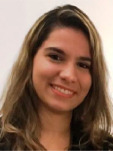
\includegraphics[width=1.2in,clip,keepaspectratio]{photos/dianne.jpg}}
~\\
\textbf{Dianne Scherly Varela de Medeiros} is a professor at the Universidade Federal Fluminense (UFF). Dianne received her Master’s degree on Telecommunications Engineering from UFF in 2013, and her D.Sc. degree on Electric Engineering from the Universidade Federal do Rio de Janeiro in 2017. Between 2015 and 2016, she had a sandwich scholarship to work on her Ph.D. Thesis on the LIP6 (Laboratoire d’Informatique de Paris 6) at Sorbonne Université, Paris, France.

\vspace{1cm}

\parpic{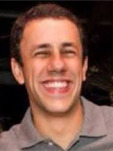
\includegraphics[width=1.2in,clip,keepaspectratio]{photos/diogo.jpg}}
~\\
\textbf{Diogo Menezes Ferrazani Mattos} is a professor at the Universidade Federal Fluminense (Niterói, Brazil). He received his degrees of D.Sc. and M.Sc. in Electrical Engineering from Universidade Federal do Rio de Janeiro, Rio de Janeiro, Brazil, in 2017 and 2012. Between 2015 and 2016, he had a sandwich scholarship to work on his Ph.D. Thesis on the LIP6 (Laboratoire d’Informatique de Paris 6) at Université Pierre et Marie Curie, Paris, France. He received a Computer and Information Engineer degree from Universidade Federal do Rio de Janeiro, in 2010, awarded with Magna Cum Laude.


\end{document}